%% BioMed_Central_Tex_Template_v1.05
%%                                      %
%  bmc_article.tex            ver: 1.05 %
%                                       %


%%%%%%%%%%%%%%%%%%%%%%%%%%%%%%%%%%%%%%%%%
%%                                     %%
%%  LaTeX template for BioMed Central  %%
%%     journal article submissions     %%
%%                                     %%
%%         <27 January 2006>           %%
%%                                     %%
%%                                     %%
%% Uses:                               %%
%% cite.sty, url.sty, bmc_article.cls  %%
%% ifthen.sty. multicol.sty		       %%
%%									   %%
%%                                     %%
%%%%%%%%%%%%%%%%%%%%%%%%%%%%%%%%%%%%%%%%%


%%%%%%%%%%%%%%%%%%%%%%%%%%%%%%%%%%%%%%%%%%%%%%%%%%%%%%%%%%%%%%%%%%%%%
%%                                                                 %%	
%% For instructions on how to fill out this Tex template           %%
%% document please refer to Readme.pdf and the instructions for    %%
%% authors page on the biomed central website                      %%
%% http://www.biomedcentral.com/info/authors/                      %%
%%                                                                 %%
%% Please do not use \input{...} to include other tex files.       %%
%% Submit your LaTeX manuscript as one .tex document.              %%
%%                                                                 %%
%% All additional figures and files should be attached             %%
%% separately and not embedded in the \TeX\ document itself.       %%
%%                                                                 %%
%% BioMed Central currently use the MikTex distribution of         %%
%% TeX for Windows) of TeX and LaTeX.  This is available from      %%
%% http://www.miktex.org                                           %%
%%                                                                 %%
%%%%%%%%%%%%%%%%%%%%%%%%%%%%%%%%%%%%%%%%%%%%%%%%%%%%%%%%%%%%%%%%%%%%%


\NeedsTeXFormat{LaTeX2e}[1995/12/01]
\documentclass[10pt]{bmc_article}    



% Load packages
\usepackage{cite} % Make references as [1-4], not [1,2,3,4]
\usepackage{url}  % Formatting web addresses  
\usepackage{ifthen}  % Conditional 
\usepackage{multicol}   %Columns
\usepackage[utf8]{inputenc} %unicode support
\usepackage{graphicx}
\usepackage{lscape}
%\usepackage[applemac]{inputenc} %applemac support if unicode package fails
%\usepackage[latin1]{inputenc} %UNIX support if unicode package fails
\urlstyle{rm}
 
 
%%%%%%%%%%%%%%%%%%%%%%%%%%%%%%%%%%%%%%%%%%%%%%%%%	
%%                                             %%
%%  If you wish to display your graphics for   %%
%%  your own use using includegraphic or       %%
%%  includegraphics, then comment out the      %%
%%  following two lines of code.               %%   
%%  NB: These line *must* be included when     %%
%%  submitting to BMC.                         %% 
%%  All figure files must be submitted as      %%
%%  separate graphics through the BMC          %%
%%  submission process, not included in the    %% 
%%  submitted article.                         %% 
%%                                             %%
%%%%%%%%%%%%%%%%%%%%%%%%%%%%%%%%%%%%%%%%%%%%%%%%%                     


%%\def\includegraphic{}
%%\def\includegraphics{}



\setlength{\topmargin}{0.0cm}
\setlength{\textheight}{21.5cm}
\setlength{\oddsidemargin}{0cm} 
\setlength{\textwidth}{16.5cm}
\setlength{\columnsep}{0.6cm}

\newboolean{publ}

%%%%%%%%%%%%%%%%%%%%%%%%%%%%%%%%%%%%%%%%%%%%%%%%%%
%%                                              %%
%% You may change the following style settings  %%
%% Should you wish to format your article       %%
%% in a publication style for printing out and  %%
%% sharing with colleagues, but ensure that     %%
%% before submitting to BMC that the style is   %%
%% returned to the Review style setting.        %%
%%                                              %%
%%%%%%%%%%%%%%%%%%%%%%%%%%%%%%%%%%%%%%%%%%%%%%%%%%
 

%Review style settings
\newenvironment{bmcformat}{\begin{raggedright}\baselineskip20pt\sloppy\setboolean{publ}{false}}{\end{raggedright}\baselineskip20pt\sloppy}

%Publication style settings
%\newenvironment{bmcformat}{\fussy\setboolean{publ}{true}}{\fussy}



% Begin ...
\begin{document}
\begin{bmcformat}


%%%%%%%%%%%%%%%%%%%%%%%%%%%%%%%%%%%%%%%%%%%%%%
%%                                          %%
%% Enter the title of your article here     %%
%%                                          %%
%%%%%%%%%%%%%%%%%%%%%%%%%%%%%%%%%%%%%%%%%%%%%%

\title{Xander: Gene Targeted Metagenomics}
 
%%%%%%%%%%%%%%%%%%%%%%%%%%%%%%%%%%%%%%%%%%%%%%
%%                                          %%
%% Enter the authors here                   %%
%%                                          %%
%% Ensure \and is entered between all but   %%
%% the last two authors. This will be       %%
%% replaced by a comma in the final article %%
%%                                          %%
%% Ensure there are no trailing spaces at   %% 
%% the ends of the lines                    %%     	
%%                                          %%
%%%%%%%%%%%%%%%%%%%%%%%%%%%%%%%%%%%%%%%%%%%%%%


\author{Jordan A Fish\correspondingauthor$^{1,2}$%
       \email{Jordan Fish\correspondingauthor - fishjord@msu.edu}%
      \and
         Yanni Sun$^2$%
         \email{Yanni Sun - yannisun@msu.edu}
       \and
         James M Tiedje$^{1,3}$%
         \email{James M Tiedje - tiedjej@msu.edu}%
       \and
         C. Titus Brown$^{2,4}$%
         \email{C. Titus Brown - ctb@msu.edu}%
         James R Cole$^1$%
         \email{James R Cole - colej@msu.edu}%
      }
      

%%%%%%%%%%%%%%%%%%%%%%%%%%%%%%%%%%%%%%%%%%%%%%
%%                                          %%
%% Enter the authors' addresses here        %%
%%                                          %%
%%%%%%%%%%%%%%%%%%%%%%%%%%%%%%%%%%%%%%%%%%%%%%

\address{%
    \iid(1)Center for Microbial Ecology, Michigan State University
    \iid(2)Department of Computer Science and Engineer, Michigan State University
    \iid(3)Department of Plant, Soil and Microbial Sciences, Michigan State University
    \iid(4)Microbiology and Molecular Genetics, Michigan State University
}%

\maketitle

%%%%%%%%%%%%%%%%%%%%%%%%%%%%%%%%%%%%%%%%%%%%%%
%%                                          %%
%% The Abstract begins here                 %%
%%                                          %%
%% The Section headings here are those for  %%
%% a Research article submitted to a        %%
%% BMC-Series journal.                      %%  
%%                                          %%
%% If your article is not of this type,     %%
%% then refer to the Instructions for       %%
%% authors on http://www.biomedcentral.com  %%
%% and change the section headings          %%
%% accordingly.                             %%   
%%                                          %%
%%%%%%%%%%%%%%%%%%%%%%%%%%%%%%%%%%%%%%%%%%%%%%


\begin{abstract}
        % Do not use inserted blank lines (ie \\) until main body of text.
        \paragraph*{Background:} Metagenomics can provide important insight in to microbial communities.  It can be used to analyze entire genomes and takes full advantage of increasing sequencing capacity. However analyzing large metagenomic datasets has proven to be very computationally challenging with even modest metagenomic datasets requiring hundreads of gigabytes to terabytes of memory to assemble with traditional assembly methods. As dataset sizes continue to increase as sequencing capacity increases new methods will be required for tackling the metagenomic assembly   problem.  In this paper, we present a method for assembling protein coding sequences for one or more genes of interest from a metagenomic dataset. This method uses a compressible graph format and only assembles targeted data to drastically reduce the amount of memory and processing time required.
        \paragraph*{Results:} Using Xander we were able to assemble contigs for two targeted gene families (rplB and nirK) from a defined community sample and a soil rihzosphere metagenomic sample.  From the defined community the assembled contigs matched the expected protein coding sequences.  Using the contigs assembled from the metagenomic sample existing nirK primers were evaluated for coverage on uncultured organisms.
        \paragraph*{Conclusions:} Gene targeted assembly enables the use gene targeted sequence analysis techniques on metagenomic datasets without requiring whole organism genomes be assembled.  Gene-targeted assembly can also aid in primer development by providing an expanded set of organisms, including uncultured ones, on which to test primer sensistivity and specificity.
\end{abstract}


\ifthenelse{\boolean{publ}}{\begin{multicols}{2}}{}




%%%%%%%%%%%%%%%%%%%%%%%%%%%%%%%%%%%%%%%%%%%%%%
%%                                          %%
%% The Main Body begins here                %%
%%                                          %%
%% The Section headings here are those for  %%
%% a Research article submitted to a        %%
%% BMC-Series journal.                      %%  
%%                                          %%
%% If your article is not of this type,     %%
%% then refer to the instructions for       %%
%% authors on:                              %%
%% http://www.biomedcentral.com/info/authors%%
%% and change the section headings          %%
%% accordingly.                             %% 
%%                                          %%
%% See the Results and Discussion section   %%
%% for details on how to create sub-sections%%
%%                                          %%
%% use \cite{...} to cite references        %%
%%  \cite{koon} and                         %%
%%  \cite{oreg,khar,zvai,xjon,schn,pond}    %%
%%  \nocite{smith,marg,hunn,advi,koha,mouse}%%
%%                                          %%
%%%%%%%%%%%%%%%%%%%%%%%%%%%%%%%%%%%%%%%%%%%%%%




%%%%%%%%%%%%%%%%
%% Background %%
%%
\section*{Background}
Metagenomics has the potential to help answer many questions but has faced scalability challenges stemming from the amount of raw sequencing data generated by metagenomic experiments\cite{pop_comparative_2004,treangen_repetitive_2011}.  Metagenomic assembly has been an area of growing interest in the past decade, with early datasets assembled using single genome assembly methods that had difficulty with metagenomic samples \cite{venter_environmental_2004,qin_human_2010}. The tendency for single genome assemblers to only assemble a few dominant organisms has been an impetus to develop metagnomic specific assembly methods\cite{namiki_metavelvet:_2012}.

We propose a gene targeted approach for assembling metagenomic datasets called Xander.  Xander is a De Bruijn Graph\cite{de_bruijn_combinatorial_1946} assembler\cite{compeau_how_2011} that uses external information to perform a guided, instead of exhaustive, traversal of the assembly graph.  Xander uses profile Hidden Markov Models (HMM) \cite{eddy_what_2004-1} to guide traversal of the assembly graph. Using an HMM, the paths most likely to code for the target gene can be extended first thus limiting the portion of the assembly graph that must be explored.  In addition to limiting the graph traversal HMMs provide a measure of how likely the resulting assembled contig comes from the supplied model.  Using a gene-targeted assembly approach allows for the use of existing functional-based analysis methods with metagenomic data.  Xander also enables researchers to examine genes involved in biologically interesting pathways without using amplicon based sequencing approaches.

Gene targeted assembly is less resource intensive and faster than traditional whole genome metagenomic assembly.  In addition to the De Bruijn Graph, only small paths relative to the graph's size must be kept in memory.  Further reduction in the memory usage are achieved by using a probabilistic data structure for holding the De Bruijn Graph in memory, a Bloom filter \cite{bloom_space/time_1970,pell_scaling_2012}.  By targeting relatively small segments of the assembly graph by using an HMM to guide assembly, the amount of the graph that must be explored during assembly is constrained, providing a speed up over whole genome approaches.

Targeted assembly of metagenomic datasets has drawn research interest and generated several approaches including EMIRGE\cite{miller_emirge:_2011} and Mira\cite{chevreux_using_2004}. EMIRGE is an expectation maximization algorithm for assembling target sequences by iterative read mapping.  The Mira assembler can perform a type of targeted assembly by using mirabait to extract out all reads that overlap with a reference set then assembling that subset of reads.  In addition to targeted-gene assembly De Bruijn Graphs have also been used as a database for a blast-like search algorithm, BlastGraph\cite{holley_blastgraph:_2012}.  Xander differs from these targeted-assembly methods, which focus on identifying reads for targeted assembly, by using a De Bruijn Graph representation of the reads.  Xander is similar to the BlastGraph approach but instead of using reads to query a De Bruijn Graph representation of the reference database, Xander queries a De Bruijn Graph representation of the reads using HMMs.
%%%%%%%%%%%%%%%%%%%%%%%%%%%%
%% Results and Discussion %%
%%
\section*{Results and Discussion}
\subsection*{HMP Mock Community}
Xander's performance was evaluated using the Human Metabiome Project's (HMP) whole genome shotgun (WGS) mock community datasets with Ribosomal Protein L2 (rplB) selected as the target gene.  \emph{rplB} was selected because it is a well conserved single copy gene.  Each organism has a single copy of the \emph{rplB} and several copies in the HMP mock community overlap by one or more 21-mer. The HMP mock community consists of 22 human gut associated microorganisms with sequenced genomes listed in Table~\ref{tab:mock_community_structure}.  The HMP mock community WGS datasets consisted of a total of one gigabase of 75 basepair Illumina sequences available from NCBI's Short Read Archive under accession numbers SRR172902, SRR172903 which were combined for all analyses.  The annotated whole genome records for each organism were downloaded from GenBank and the Coding Sequence (CDS) annotation was extracted.

The combined dataset was quality filtered as described below, a summary of the trimming results is contained in Table~\ref{tab:trimming_stats}.  A Bloom filter was built from the combined dataset in 8 minutes 41 seconds with an estimated 0.001\% false positive rate.  The Bloom filter was built with a k-mer size of 21 using four hash functions and was one gigabyte in size.

To evaluate the coverage of the HMP mock community dataset the combined read set was mapped to the whole genome sequences for all the organisms using Bowtie2\cite{langmead_fast_2012} summarized in Fig~\ref{fig:bowtie_mapping}.  Two organisms were not targeted for assembly: Candida albicans is a eukaryote and hence does not have a copy of bacterial \emph{rplB} and Listeria monocytogenes since only a hand full of reads mapped to it's \emph{rplB} region.

The starting vertices for Xander's search were selected by first aligning the reference genomes' translated \emph{rplB} sequences to the \emph{rplB} model used for searching.  The protein alignment was then used to align the nucleotide sequences for each reference.  For each \emph{rplB} nucleotide reference sequence, the first consecutive 21 nucleotides aligning to the rplB model (e.g. without gaps or insertions), along with the model position the first resiude occupied were used as the search start points.  A total of 20 starting vertices were selected, one from each of the 20 organisms selected.

Xander was then run on the selected starts and a summary of the results are show in Table~\ref{tab:xander_hmp_summary}.  Using the HMP mock community dataset with the start points selected Xander was able to assemble 20 \emph{rplB} gene sequences with an average protein-protein identity to the reference gene of 90\%.  About half of the resulting sequences were partial assemblies, which due to cuts in the assembly graph caused by zero coverage for parts of the reference genomes which can be seen in the average coverage data in Table~\ref{tab:xander_hmp_summary} and in detail in Supplemental 1.  Since several of the organisms overlapped by at least one 21-mer the paths in the assembly graph crossed which combined with sequencing errors lead to the differences seen between the expected protein sequence and assembled contig.

\subsection*{Primer Validation with Rizosphere Metagenome}
Xander was used with a soil metagenomic dataset to assembly \emph{nirK} sequences.  The metagenomic sample was taken from a GLBRC test plot at Kellogg Biological Station and sequenced with the Illumina GAII sequencer.  The dataset contained approximately 530 million 100 basepair reads.  The sequence data was obtained after quality trimming was performed. The De Bruijn Graph was constructed in nine hours with a k value of 30 using a Bloom filter size of 32GB, using four hash functions, and with an estimated false positive rate of 0.5\%.

These assembled sequences were then analyzed to test the sensitivity and specificity of two sets of \emph{nirK} primers, nirK1F:nirK5R \cite{braker_development_1998} and F1Cu:R5Cu \cite{hallin_pcr_1999}.  The coverage of the two sets of primers was evaluated on published \emph{nirK} sequences using the FunGene Repository.  The coverage of the two primers was also evaluated against the \emph{nirK} sequences assembled by Xander from the MSR2 dataset.  The results of the coverage analysis are show in Table~\ref{tab:nirk_primer_coverage}.  The nirK1F primer spanned a region maked as an insert in the HMM used for assembly and primer analysis which caused the gaps seen in Fig~\ref{fig:nirk_primer_conservation}.

\subsection*{Cuts in the Assembly Graph}

In addition to producing partial assemblies, cuts in the assembly graph can stop the search from terminating in a reasonable amount of time. If there is no path to the end of the model the A* search devolves in to an exhaustive traversal of the graph, something we specifically want to avoid.  To handle these cases, two heuristic pruning methods were developed based on the log odds ratio comparing the probability the current path was generated by the HMM or a null model described in the Methods below.  The effects of the different pruning methods can be seen in Fig~\ref{fig:comp_pruning_techniques}.  By making the pruning heuristic more strict Xander considers far fewer nodes enabling faster searching and discarding non-target path segments.

%%%%%%%%%%%%%%%%%%%%%%
\subsection*{Conclusions}
Xander is more sensitive than whole genome assembly methods and more specific than individual read-based approaches for functional analysis.  Using an assembly based approach provides more context from which to make a classification decision as to whether a stretch of sequence belongs to the target gene family or not.  Using HMM probabilities to guide local assembly helps to ensure the most relevant paths are explored to assemble sequences most likely to code for the target gene.
  
%%%%%%%%%%%%%%%%%%
\section*{Methods}
\subsection*{Xander Gene-Targeted Assembly}
\subsubsection*{Graph Structure}
A novel graph structure was created that combined a De Bruijn Graph (DG) and HMM together in a single combined assembly graph (CG) for assembling genes of interest.  A vertex in CG is created for every pair of vertices u, v in DG and HMM:
\[ \forall (u,v)\, u\in \textnormal{DG, }v\in \textnormal{HMM} \] each vertex in CG combines the information in $u$ and $v$.
The total number of vertices in CG will be \[|V(DG)| * |V(HMM)|\] where V(G) is the vertex set of the graph G.  Vertices in CG are generated as needed to reduce the memory requirements.

The edge set $E(CG)$ was defined as follows: suppose $w_i$, and $w_j$ \(\in V(CG) \) and were made by combining vertices $v_i$ with $u_i$ and $v_j$ with $u_j$ respectively with $v$ vertices from the De Bruijn Graph and $u$ vertices from the HMM.
\[\overrightarrow{w_iw_j} \in E(\textnormal{CG}) \leftrightarrow \overrightarrow{v_iv_j} \in E(\textnormal{DG})\textnormal{ and } \overrightarrow{u_iu_j} \in E(\textnormal{HMM})\].
That is, an edge exists in CG if and only if an edge connects the vertices they were created by combining. The weight of an edge \overrightarrow{uv} in CG are the defined as sum of the transition and emission probabilities taken from the HMM.  
\[ weight(\overrightarrow{uv}) = P_{transition}(u \rightarrow v) + P_{emission}(v) \]
The emission symbol is the unique character in the K-mer contained in v.

The De Bruijn Graph is constructed in nucleotide space regardless of whether the HMM is modeling protein or nucleotide sequences. When searching with a protein HMM the De Bruijn Graph is traversed in protein space by walking three nodes in any one direction at a time.  The emission symbol then becomes the three unique characters at the end of the K-mer translated to protein.  The codon reading frame is fixed based on the vertex chosen to begin graph traversal.

\subsubsection*{Seed Identification}
Xander includes two ways to identify seed kmers from which to start searching.  Both methods use a representative reference set of aligned sequences from the target gene family.  The k-mer and the model position from the aligned reference, and implicit match HMM state are combined to form a search starting vertex in CG.

The first seed identification approach is an exact seed matching approach. The reference sequences were broken up in to K-mers and stored in a hash table. Each read was then decomposed into K-mers that were then looked up in the hash of the references K-mers.  For use with a protein HMM a seed length of $\lfloor K/3\rfloor$ was used and input reads were translated in to all six reading frames. When assembling multiple target gene families the reference sets can be combined together into a single hash so that potential search starts can be identified in a single pass over the reads.

The second seed identification approach combines the seed identification and searching in to one step.  The aligned reference file is provided to the BasicSearch program which then decomposes all the reference reads in to k-mers.  When protein gene family is being targeted the references are broken up in to $k/3$ length words and back translated in to all possible nucleotide k-mers that translate to the reference protein word.  The Bloom filter is then queried for each reference k-mer, any k-mers identified are then used as a starting point for a search.  

\subsubsection*{Assembly Approach}
Assemblies in Xander are done using the A* search algorithm\cite{hart_formal_1968} for finding paths through the CG.  The A* implementation in Xander was  modified to find the highest scoring path instead of the lowest cost path. The set of goal vertices is defined as any vertex in the last model position that is in the match or delete state.  The scoring function for a path P is defined as: 
\[S(P) = \sum_{i=0}^{|P|}w(P_iP_{i+1})\] 
where w(\ldots) is the weight of the edge between two vertices in P.  By using the transition and emission probabilities from the HMM and selecting the highest scoring path through the graph the search is analagous to the Viterbi Decoding\cite{viterbi_error_1967} algorithm.

The heuristic cost function for a vertex v is defined as:
\[h(v) = P_{v_{state}\rightarrow match} + \sum_{i=v_{model position} + 1}^{M}P_{match\rightarrow match}(i, i + 1)\]
the sum of the most likely state transitions from a v's state to the end of the model. Where $P$ is the probability of the given transition and M is the length of the HMM.

To ensure The log-odds edge weights used by the heuristic score and scoring function were monotonic the following transformation is applied to every edge in CG:
\[ w(\overrightarrow{uv}) = w(\overrightarrow{uv}) - max(P_{emission}(v_{HMM state})) \quad u_{HMM state} \ne i\]
Since this heuristic score will never overestimate the actual score it meets the admissibility criteria for A*, and additionally since the scoring function is monotonic a closed set is not required.

Since search starting vertices can be in any model position, not just the beginning of the model, a second HMM is built from the reverse of the seed alignment used to build the forward HMM.  Using this reverse model Xander can traverse paths in both directions from a starting vertex.  The contigs generated by each search direction are reported seperately; a tool is included with Xander to combine the two contigs fragments in to a single contig.

\subsubsection*{K Shortest Paths}
A Kth shortest path algorithm\cite{yen_finding_1971} to find multiple high scoring paths from a single starting vertex.  Yen's algorithm iteratively finds the shortest path, then 2nd shortest path to the kth shortest path.  This is sped up by the observation that the $i$th shortest path in the sequence must branch from one of the $i-1$ shortest paths already identified.  Yen's algorithm can be further improved by the observation that the $i$th shortest path must branch from it's parent $j$ after the point $j$ branched from it's parent\cite{lawler_procedure_1972}.  The version of Yen's algorithm implemented in Xander was modified to discard paths that did not contain unseen kmers.  In this way each of the K shortest paths found contain new information.

\subsubsection*{Prunning Unproductive Paths}
Xander implements a path pruning heuristics to remove paths that are unlikely to yield contigs that match the model well.  When a node is opened the probability of the path to that point is calculated and compared to the probability of the path being generated from a null model (cite hmmer2 null model) and the node is discarded if the log odds ratio is below a threshold value $\theta$. In the event a search terminates before reaching the end of the model, the intermediate node with the highest bits saved score is returned.  This heuristic pruning is done in addition to the A* search. The log-odds-ratio threshold can be tuned using a command line switch to balance the trade-off between sensitivity and running time.

\subsection*{Data Processing}
\subsubsection*{Quality Filtering}
Read quality filtering was performed by trimming reads at quality score 2 as recommended by Illumina (CASAVA1.7 User Guide) using the SequenceTrimmer tool in the ReadSeq package (\url{http://github.com/rdpstaff/ReadSeq}.

\subsubsection*{HMM Construction}
The HMMs were built using the seed sequences from the Functional Gene Repository (cite frontiers article).  These seed sequences were used to build an HMM for each gene using a modified version of HMMER3 using the \begin{verbatim}--enone\end{verbatim} option to disable sequence weighting. HMMER3's default settings were tuned for detecting remote paralogs\cite{johnson_division_2006} where Xander is targeting close homologs.  The default priors sometimes caused extensive searching of nonproductive insert and delete paths. HMMER3's source code was modified to change the prior probabilities for the $delete \rightarrow match$ and $insert \rightarrow match$ transitions to 95\% probability, $delete \rightarrow delete$ and $insert \rightarrow insert$ transitions to 5\% probability.  The modifications to HMMER3 are available as a patch file against version 3.0.

\subsubsection*{Primer Coverage Analysis}
To test the coverage of primers on public sequences the ProbeMatch tool in the FunGene Repository was used.  To test the coverage of primers on sequences assembled using Xander first the primer region was located in the HMM.  This was done by aligning a randomly chosen public sequence with a perfect match to each primer to the HMM for the target family.  The protein alignment was back-translated to the nucleotide sequence and then the model position of the start and end of each primer region was then recorded.  The assembled sequences were then aligned to the HMM for the target family and used to back translate the alignment to the assembled nucleotide sequences.  For all assembled sequences that covered each primer region, that region was extracted and used to generate a sequence conservation logo \cite{schneider_sequence_1990}.  Finally the coverage of each primer was computed by dividing the number of assembled sequences that matched the primer by the number of assembled sequences containing the primer region.

\subsection*{Implementation and Avaliability}
Xander was implemented in the Java programming language and is distributed under the terms of the GPLv3 License available from \url{https://github.com/rdpstaff/Xander-HMMgs}.  Xander uses a Bloom filter to store a compressed representation of the De Bruijn Graph. Xander consists of three primary tools; one for building a Bloom filter De Bruijn Graph, a tool for identifying starting positions, the core search tool. Support programs and scripts are also included with Xander for manipulating file formats, combining contig fragments and filtering Xander results.

Any of the tools can be replaced with a $3^{rd}$ party tool using difference heuristics as long as the resulting file matches the expected format.  For example the starting vertex identification can be replaced with a $3^{rd}$ party tool so long as the resulting file contains the starting kmer and starting model position.

The scripts used to perform analyses for this paper are available from \url{http://github.com/fishjord/2013-xander-paper}.
    
%%%%%%%%%%%%%%%%%%%%%%%%%%%%%%%%
\section*{Authors contributions}
    Text for this section \ldots

    

%%%%%%%%%%%%%%%%%%%%%%%%%%%
\section*{Acknowledgements}
  \ifthenelse{\boolean{publ}}{\small}{}
  Text for this section \ldots


 
%%%%%%%%%%%%%%%%%%%%%%%%%%%%%%%%%%%%%%%%%%%%%%%%%%%%%%%%%%%%%
%%                  The Bibliography                       %%
%%                                                         %%
%%  Bmc_article.bst  will be used to                       %%
%%  create a .BBL file for submission, which includes      %%
%%  XML structured for BMC.                                %%
%%                                                         %%
%%                                                         %%
%%  Note that the displayed Bibliography will not          %% 
%%  necessarily be rendered by Latex exactly as specified  %%
%%  in the online Instructions for Authors.                %% 
%%                                                         %%
%%%%%%%%%%%%%%%%%%%%%%%%%%%%%%%%%%%%%%%%%%%%%%%%%%%%%%%%%%%%%


{\ifthenelse{\boolean{publ}}{\footnotesize}{\small}
 \bibliographystyle{bmc_article}  % Style BST file
  \bibliography{references.bib} }     % Bibliography file (usually '*.bib' ) 

%%%%%%%%%%%

\ifthenelse{\boolean{publ}}{\end{multicols}}{}

%%%%%%%%%%%%%%%%%%%%%%%%%%%%%%%%%%%
%%                               %%
%% Figures                       %%
%%                               %%
%% NB: this is for captions and  %%
%% Titles. All graphics must be  %%
%% submitted separately and NOT  %%
%% included in the Tex document  %%
%%                               %%
%%%%%%%%%%%%%%%%%%%%%%%%%%%%%%%%%%%

%%
%% Do not use \listoffigures as most will included as separate files

\section*{Figures}
\subsection*{Figure 1 - HMP Mock Community Read Mapping}
  \label{fig:bowtie_mapping}
  Percentage of reads mapped (unnormalized) to the reference organism.  For organisms with more than one chromosome only the reads mapping to the chromosome containing the rplB gene were counted.
  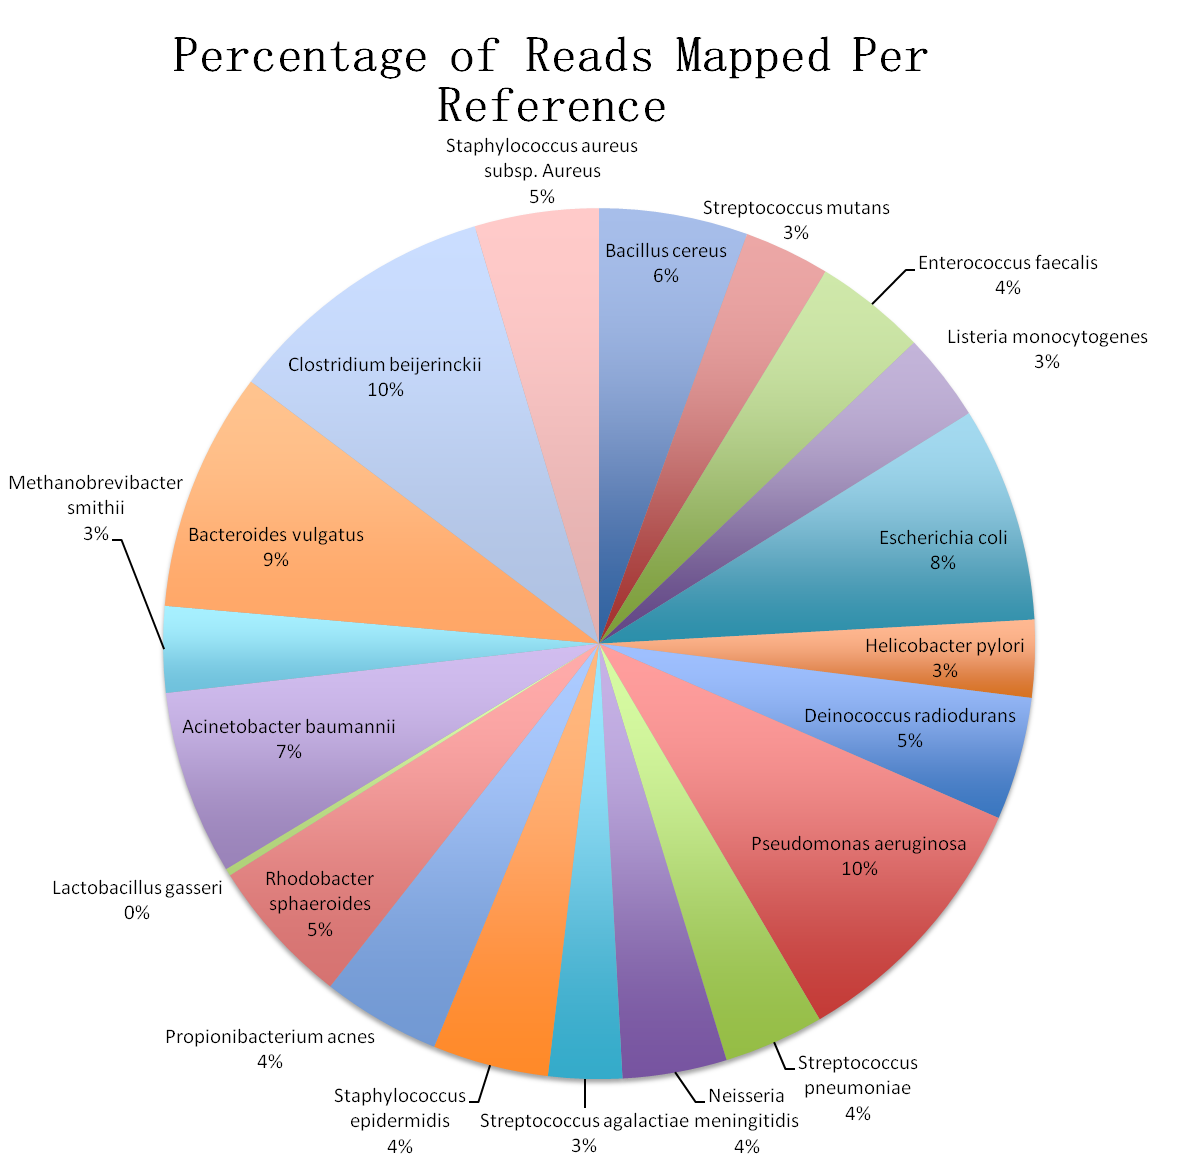
\includegraphics[width=117mm]{figs/hmp_mock_community_mapping_chart.png}
\subsection*{Figure 2 - Comparision of pruning heursitics}
  \label{fig:comp_pruning_techniques}
  Effect of cuts in the assembly graph on resulting contig plus effectiveness of different heuristic path pruning techniques.
  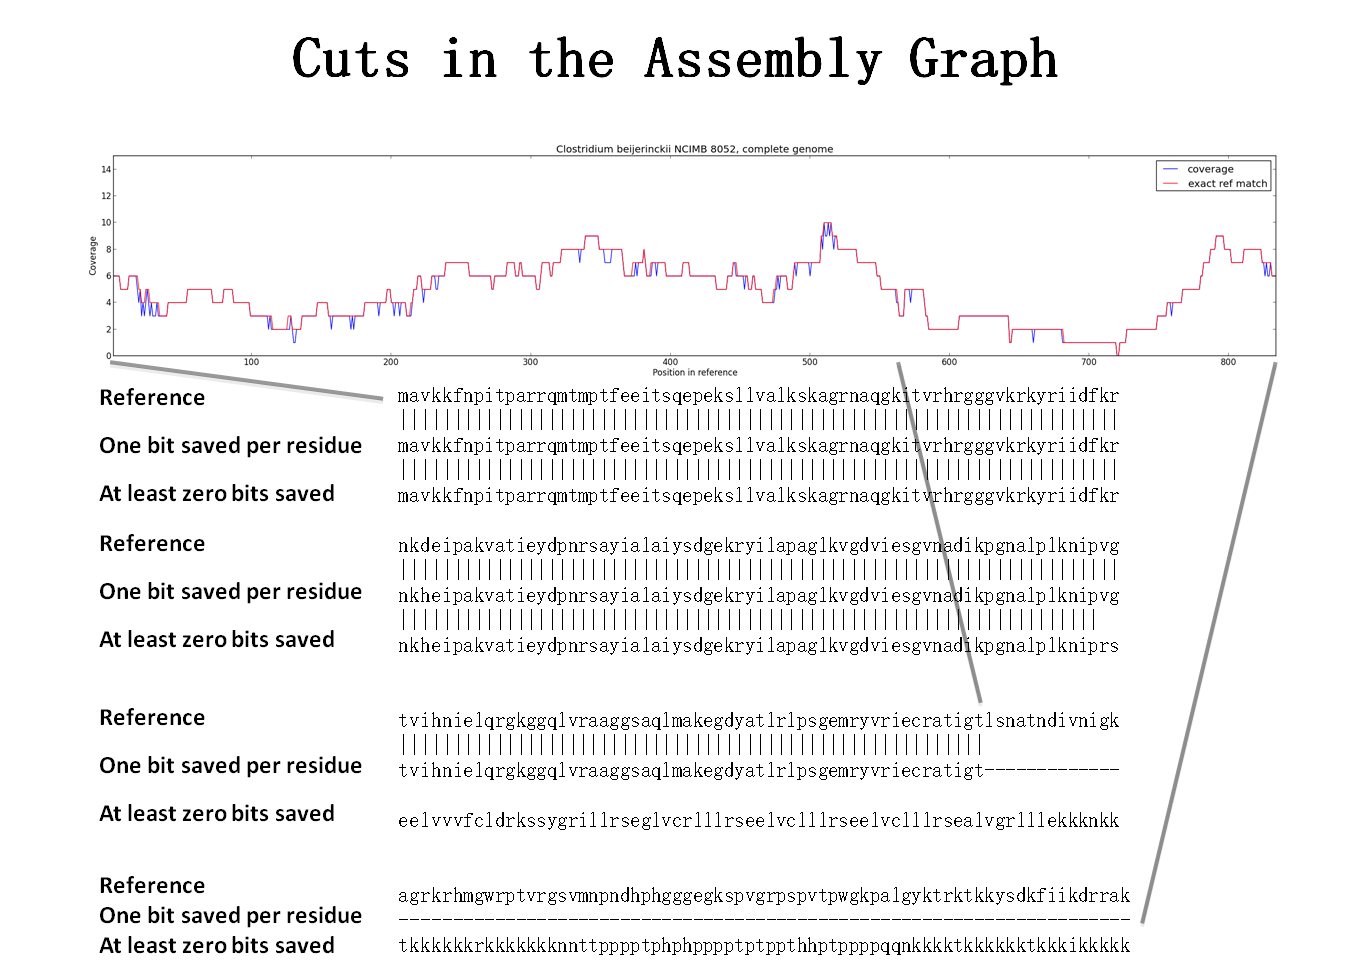
\includegraphics[width=117mm]{figs/pruning_heuristics.png}
\subsection*{Figure 3 - Combined Graph Structure}
  \label{fig:combined_graph}
  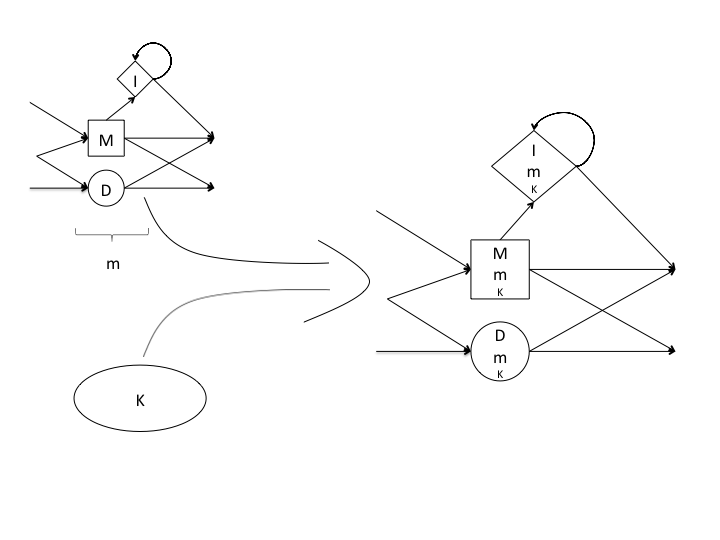
\includegraphics[width=117mm]{figs/combined_graph.png}
\subsection*{Figure 4 - Sequence conservation of \emph{nirK} primer regions}
	\label{fig:nirk_primer_conservation}
	Sequence conservation logos for the primer regions of the \emph{nirK} sequences assembled using Xander from the MSR2 dataset. a) nirK1F b) nirK5R c) F1aCu d) R3Cu.
	\par
	a. \par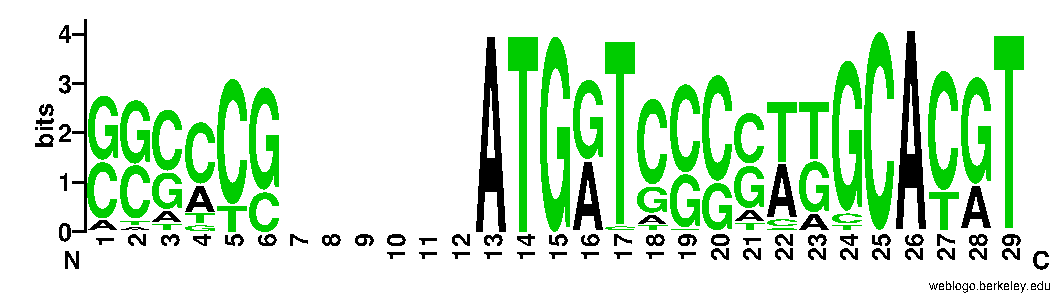
\includegraphics[width=5cm]{figs/nirK1F_logo.pdf}
	b. \par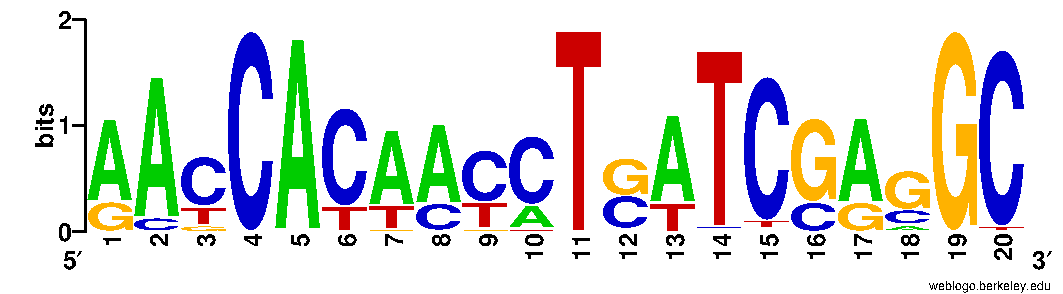
\includegraphics[width=5cm]{figs/nirK5R_logo.pdf}
	c. \par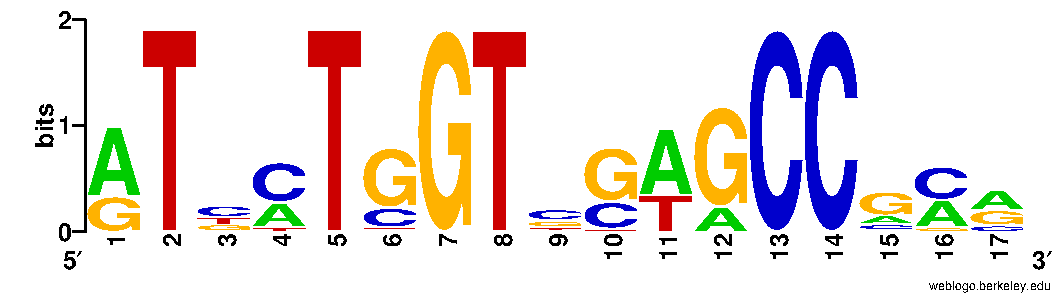
\includegraphics[width=5cm]{figs/F1aCu_logo.pdf}
	d. \par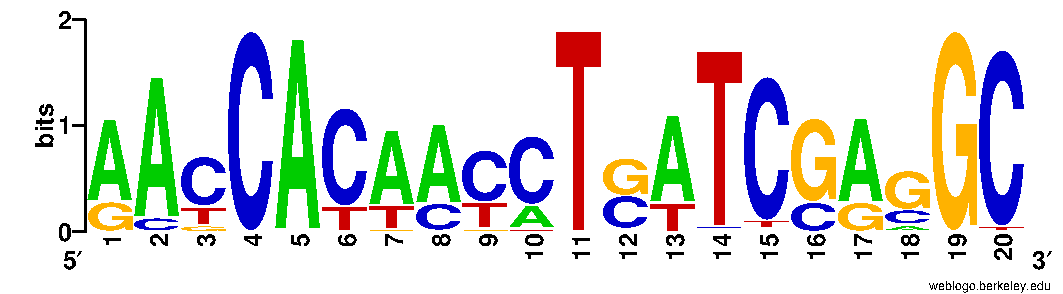
\includegraphics[width=5cm]{figs/R3Cu_logo.pdf}
	


%%%%%%%%%%%%%%%%%%%%%%%%%%%%%%%%%%%
%%                               %%
%% Tables                        %%
%%                               %%
%%%%%%%%%%%%%%%%%%%%%%%%%%%%%%%%%%%

%% Use of \listoftables is discouraged.
%%
\section*{Tables}
  \subsection*{Table 1 - HMP Mock Community Composition}
  \label{tab:mock_community_structure}
  Organisms in the HMP mock community and accession number of the GenBank record from which annotations were harvested. \\
  $^\dagger$ indicates genome records with incomplete annotations, annotations from another assembly of a synonmous strain (the accession number in parathesis) were used instead.
  $^*$ indicates genomes that were removed from the final analysis.
    \par
    \mbox{\tiny
      \begin{tabular}{|c|p{5cm}|c|}
	\hline
        Organism Name & Strain & Accession Number \\
	\hline
        Streptococcus mutans & NN2025 DNA & NC\_003028 (AP010655) $^\dagger$ \\
        Listeria monocytogenes$^*$ & L99 serovar 4a & NC\_003210 (FM211688)$^\dagger$ \\
        Acinetobacter baumannii & ATCC 17978 & NC\_009085.1 \\
        Acinetobacter baumannii & ATCC 17978 plasmid pAB1 & NC\_009083.1 \\
        Acinetobacter baumannii & ATCC 17978 plasmid pAB2 & NC\_009084.1 \\
        Actinomyces odontolyticus & ATCC 17982 Scfld020 \& Scfld021  &   DS264586.1 \\
        Actinomyces odontolyticus & ATCC 17982 Scfld020  & DS264585.1 \\
        Bacillus cereus & ATCC 10987 & AE017194.1 \\
        Bacillus cereus & ATCC 10987 plasmid pBc10987 & NC\_005707.1 \\
        Bacteroides vulgatus & ATCC 8482 & NC\_009614.1 \\
        Candida albicans$^*$ & SC5314 Assembly 21 & N/A \\
        Clostridium beijerinckii & NCIMB 8052 &   NC\_009617.1 \\
        Deinococcus radiodurans & R1 chromosome 1 &     NC\_001263.1 \\
        Enterococcus faecalis & OG1RF chromosome &  ABPI01000001.1 \\
        Escherichia coli & K12 &  NC\_000913.2 \\
        Helicobacter pylori & 26695 &     NC\_000915.1 \\ 
        Lactobacillus gasseri & ATCC 33323 &      NC\_008530.1 \\
        Methanobrevibacter smithii & ATCC 35061 &  NC\_009515.1 \\
        Neisseria meningitidis & MC58 &   NC\_003112.2 \\
        Propionibacterium acnes & KPA171202 &     NC\_006085.1 \\
        Pseudomonas aeruginosa &  PAO1 &   NC\_002516.2 \\
        Rhodobacter sphaeroides & 2.4.1 chromosome 1 &  NC\_007493.1 \\
        Rhodobacter sphaeroides & 2.4.1 chromosome 2 &  NC\_007494.1 \\
        Rhodobacter sphaeroides & 2.4.1 plasmid A, partial sequence &      NC\_009007.1 \\
        Rhodobacter sphaeroides & 2.4.1 plasmid B &     NC\_007488.1 \\
        Rhodobacter sphaeroides & 2.4.1 plasmid C &     NC\_007489.1 \\
        Rhodobacter sphaeroides & 2.4.1 plasmid D &     NC\_007490.1 \\
        Rhodobacter sphaeroides & 2.4.1 plasmid E &     NC\_009008.1 \\
        Staphylococcus aureus subsp. aureus & USA300\_TCH1516 &    NC\_010079.1 \\
        Staphylococcus aureus subsp. aureus & USA300\_TCH1516 plasmid pUSA300HOUMR &      NC\_010063.1 \\
        Staphylococcus aureus subsp. aureus & USA300\_TCH1516 plasmid pUSA01-HOU &       NC\_012417.1 \\
        Staphylococcus epidermidis & ATCC 12228 &  NC\_004461.1 \\
        Staphylococcus epidermidis & ATCC 12228 plasmid pSE-12228-06 &   NC\_005003.1 \\
        Staphylococcus epidermidis & ATCC 12228 plasmid pSE-12228-05 &   NC\_005004.1 \\
        Staphylococcus epidermidis & ATCC 12228 plasmid pSE-12228-04 &   NC\_005005.1 \\
        Staphylococcus epidermidis & ATCC 12228 plasmid pSE-12228-03 &   NC\_005006.1 \\
        Staphylococcus epidermidis & ATCC 12228 plasmid pSE-12228-02 &   NC\_005007.1 \\
        Staphylococcus epidermidis & ATCC 12228 plasmid pSE-12228-01 &   NC\_005008.1 \\
        Streptococcus agalactiae & 2603V/R & NC\_004116.1 \\
        Streptococcus pneumoniae & TIGR4 & NC\_003028.3 \\
	\hline
      \end{tabular}
      }
  \subsection*{Table 2 - HMP Trimming summary}
	\label{tab:trimming_stats}
	Summary of the quality filtering results on the HMP Mock Community.  Half the reads had at least one base removed from the 3' end. 17403 reads had no bases left after trimming and were removed.
	\par
	\mbox{
	\begin{tabular}{|c|c|c|c|}
		\hline
		& Total sequences & Total Bases & Average Length \\
		\hline
		Before Trimming & 14494884 & 1037 MB & 75 \\
		After Trimming & 14477481 & 905 MB & 65.5 \\
		\hline
	\end{tabular}
	}
  \subsection*{Table 3 - Summary of Xander results for the HMP Mock community}
    \label{tab:xander_hmp_summary}
    Output of running Xander on the HMP mock community WGS dataset.  The forward and reverse searches for each reference are combined in a single row in the table with the total time for each direction's search reported.  The fragment nats (probability log base e) represent the score A* was optimizing on while the bits saved reflects the probability the sequence comes from the HMM.  The average coverage of the \emph{rplB} region computed by bowtie mapping for each reference is also reported.
    \par
    \begin{landscape}
    \mbox{\tiny
      \begin{tabular}{|c|p{1cm}|p{1cm}|p{1cm}|p{1.5cm}|p{1.5cm}|p{1.5cm}|p{1.5cm}|p{1cm}|p{1.5cm}|}
        \hline
        Reference Organism & Reference Length & Starting State & Protein Length & left nats & left bits saved & right nats & rightbits saved & Search Time (s) & Average coverage (by bowtie2 mapping) \\ 
        \hline
        Bacillus cereus & 274 & 250 & 31 & -14.744 & 20 & -8.216 & 68.66 & 0.123 & 1.07 \\
        Streptococcus mutans & 263 & 256 & 283 & -14.55 & 62.36 & -66.953 & 815.82 & 1.933 & 26.84 \\
        Enterococcus faecalis & 277 & 270 & 284 & -11.49 & 123.61 & -69.908 & 859.67 & 1.758 & 2.08 \\
        Escherichia coli & 274 & 271 & 61 & -3.263 & 25.38 & -21.885 & 151.62 & 1.749 & 10.16 \\
        Helicobacter pylori & 277 & 271 & 66 & -1.742 & 27.57 & -42.965 & 141.71 & 0.005 & 6.7 \\
        Deinococcus radiodurans & 276 & 271 & 282 & -3.17 & 725.5 & -113.486 & 802.01 & 6.192 & 55.86 \\
        Pseudomonas aeruginosa & 274 & 271 & 41 & -1.983 & 27.22 & -20.531 & 86.73 & 0.005 & 3.8 \\
        Streptococcus pneumoniae & 278 & 270 & 284 & -15.275 & 18.16 & -72.054 & 856.43 & 7.52 \\
        Neisseria meningitidis & 278 & 271 & 23 & -4.065 & 24.22 & -8.74 & 50.93 & 0.001 & 6.43 \\
        Streptococcus agalactiae & 263 & 270 & 284 & -14.878 & 18.73 & -71.657 & 857 & 1.983 & 1.78 \\
        Staphylococcus epidermidis & 278 & 271 & 284 & -1.652 & 27.7 & -73.829 & 858.71 & 4.571 & 41.23 \\
        Propionibacterium acnes & 279 & 271 & 282 & -1.108 & 28.49 & -106.232 & 812.45 & 4.509 & 7.19 \\
        Rhodobacter sphaeroides & 280 & 271 & 281 & -4.922 & 22.98 & -174.453 & 714.31 & 3.515 & 33.66 \\
        Lactobacillus gasseri & 277 & 193 & 2 & -21.946 & 15.45 & -26.169 & 51.91 & 0.001 & 0.09 \\
        Acinetobacter baumannii & 243 & 238 & 284 & -32.284 & 84.36 & -61.043 & 771.09 & 0.732 & 12.44 \\
        Methanobrevibacter smithii & 242 & 177 & 17 & -22.914 & 12.43 & -13.467 & 24.65 & 0.001 & 13.43 \\
        Bacteroides vulgatus & 274 & 271 & 281 & -2.035 & 27.15 & -173.271 & 717.96 & 1.022 & 9.72 \\
        Clostridium beijerinckii & 278 & 271 & 201 & -2.702 & 26.19 & -82.677 & 552.85 & 42.109 & 4.87 \\
        Staphylococcus aureus subsp. aureus & 278 & 269 & 284 & -5.063 & 34.49 & -74.807 & 853.08 & 3.192 & 50.18 \\
        \hline
      \end{tabular}
    }
      \end{landscape}
	\subsection*{Table 4 - \emph{nirK} Primer Coverage}
	\label{tab:nirk_primer_coverage}
	Coverage of published \emph{nirK} primers nirK1F, nirK5R, F1aCu and R3Cu on \emph{nirK} sequences assembled from the MSR2 soil rizosphere metagenomic dataset and FunGene Repository (7,643 \emph{nirK} sequences from release 7.2) allowing up to two mismatches.
	\par
	\mbox{\tiny
	\begin{tabular}{|c|c|cc|ccc|}
	\hline
	& & \multicolumn{2}{|c|}{FunGene Repository} & \multicolumn{3}{|c|}{MSR2} \\
	Primer & Sequence & Number of Hits & Coverage & Covering region & Matching Primer & Coverage \\
	\hline
	nirK1F & GGMATGGTKCCSTGGCA & 1084 & 14\% & 113 & 1 & 1\% \\
	nirK5R & GCCTCGATCAGRTTGTGGTT & 3656 & 48\% & 118 & 67 & 57\% \\
	F1aCu & ATCATGGTSCTGCCGCG & 3247 & 42\% & 125 & 19 & 15\% \\
	R3Cu & GCCTCGATCAGRTTGTGGTT & 3656 & 48\% & 118 & 67 & 58\% \\
	\hline
	\end{tabular}
	}


%%%%%%%%%%%%%%%%%%%%%%%%%%%%%%%%%%%
%%                               %%
%% Additional Files              %%
%%                               %%
%%%%%%%%%%%%%%%%%%%%%%%%%%%%%%%%%%%

\section*{Additional Files}
  \subsection*{Additional file 1 --- Sample additional file title}
    Additional file descriptions text (including details of how to
    view the file, if it is in a non-standard format or the file extension).  This might
    refer to a multi-page table or a figure.


\end{bmcformat}
\end{document}







